\paragraph{CPSs (1)}

The graph below is a constraint graph for a CSP that has only binary constraints. Initially, no variables have been assigned.
\\\\
For each of the following scenarios, mark all variables for which the specified filtering might result in their domain being changed. 

\begin{center}
    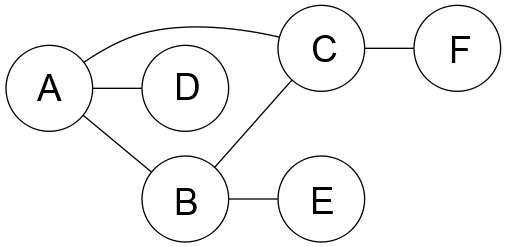
\includegraphics[scale=.43]{figures/domainFiltering.png}
\end{center}



\begin{enumerate}

\item A value is assigned to A. Which domains might be changed as a result of running forward checking for A? (\textbf{10 points})

\vspace{2cm}

\item A value is assigned to A, and then forward checking is run for A. Then a value is assigned to B. Which domains might be changed as a result of running forward checking for B? (\textbf{10 points})

\vspace{2cm}


\item A value is assigned to A. Which domains might be changed as a result of enforcing arc consistency after this assignment? (\textbf{10 points})

\vspace{2cm}


\item A value is assigned to A, and then arc consistency is enforced. Then a value is assigned to B. Which domains might be changed as a result of enforcing arc consistency after the assignment to B? (\textbf{10 points})

\vspace{2cm}


\end{enumerate}

\newpage

\paragraph{CPSs (2)}

After years of struggling through mazes, Pacman has finally made peace with the ghosts, Blinky, Pinky, Inky, and Clyde, and invited them to live with him and Ms. Pacman. The move has forced Pacman to change the rooming assignments in his house, which has 6 rooms. He has decided to figure out the new assignments with a CSP in which the variables are Pacman \textbf{(P)}, Ms. Pacman \textbf{(M)}, Blinky \textbf{(B)}, Pinky \textbf{(K)}, Inky \textbf{(I)}, and Clyde \textbf{(C)}, the values are which room they will stay in, from 1-6, and the constraints are:\\
\begin{table}[h]
\centering
\caption{Constraints}
\begin{tabular}{ll}
i) No two agents can stay in the same room&\\
ii) \textbf{P} $>$ 3 &
vi) \textbf{B} is even\\
iii) \textbf{K} is less than \textbf{P}&
vii) \textbf{I} is not 1 or 6\\
iv) \textbf{M} is either 5 or 6&
viii) $\vert$\textbf{I}-\textbf{C}$\vert$ = 1\\
v) \textbf{P} $>$ \textbf{M}&
ix) $\vert$\textbf{P}-\textbf{B}$\vert$ = 2
\end{tabular}
\end{table}


\begin{enumerate}
  \item {\bf Unary constraints} On the grid below cross out the values from each domain that are eliminated by enforcing unary constraints. (\textbf{10 points})

  \begin{table}[h]
\centering
\caption{}
\begin{tabular}{ccccccc}
P & 1 & 2 & 3 & 4 & 5 & 6\\
B & 1 & 2 & 3 & 4 & 5 & 6\\
C & 1 & 2 & 3 & 4 & 5 & 6\\
K & 1 & 2 & 3 & 4 & 5 & 6\\
I & 1 & 2 & 3 & 4 & 5 & 6\\
M & 1 & 2 & 3 & 4 & 5 & 6\\
\end{tabular}
\end{table}

\vspace{2cm}


\item {\bf MRV}
According to the Minimum Remaining Value (MRV) heuristic, which variable should be assigned to first? (\textbf{10 points})

\newpage

\item {\bf Forward Checking}
For the purposes of decoupling this problem from your solution to the
previous problem, assume we choose to assign P first, and assign it the value 6. What are the resulting domains after enforcing unary constraints (from part i) and running forward checking for this assignment? (\textbf{15 points})

\begin{table}[h]
\centering
\caption{}
\begin{tabular}{ccccccc}
P &   &   &   &  &   &  6\\
B & 1 & 2 & 3 & 4 & 5 & 6\\
C & 1 & 2 & 3 & 4 & 5 & 6\\
K & 1 & 2 & 3 & 4 & 5 & 6\\
I & 1 & 2 & 3 & 4 & 5 & 6\\
M & 1 & 2 & 3 & 4 & 5 & 6\\
\end{tabular}
\end{table}

\vspace{1cm}


\item {\bf Iterative Improvement}
Instead of running backtracking search, you decide to start over and run
iterative improvement with the min-conflicts heuristic for value selection. Starting with the following assignment:\\\\
P:6, B:4, C:3, K:2, I:1, M:5\\\\
First, for each variable write down how many constraints it violates in the table below.\\
Then, in the table on the right, for all variables that could be selected for assignment, put an x in any box that corresponds to a possible value that could be assigned to that variable according to min-conflicts. When marking next values a variable could take on, only mark values different from the current one. (\textbf{25 points})

\begin{center}
\begin{tabular}{cc}
\begin{tabular}{|c|c|}
\hline
Variable & \# violated\\
\hline
P& \\
\hline
B& \\
\hline
C& \\
\hline
K& \\
\hline
I& \\
\hline
M& \\
\hline
\end{tabular} \hspace{2cm}&
\begin{tabular}{|c|c|c|c|c|c|c|}
\hline
&1&2&3&4&5&6\\
\hline
P& & & & & &\\
\hline
B& & & & & &\\
\hline
C& & & & & &\\
\hline
K& & & & & &\\
\hline
I& &  & &  & &\\
\hline
M& & & & & &\\
\hline
\end{tabular}
\end{tabular}
\end{center}

\end{enumerate}